
%%let's use a standard format for the discussion
%https://www.ncbi.nlm.nih.gov/pmc/articles/PMC4548568

%The introductory paragraph contains the main idea of performing the study in question. Without repeating ‘Introduction’ section of the manuscript, the problem to be addressed, and its updateness are analysed. The introductory paragraph starts with an undebatable sentence, and proceeds with a part addressing the following questions as 1) On what issue we have to concentrate, discuss or elaborate? 2) What solutions can be recommended to solve this problem? 3) What will be the new, different, and innovative issue? 4) How will our study contribute to the solution of this problem An introductory paragraph in this format is helpful to accomodate reader to the rest of the Discussion section. However summarizing the basic findings of the experimental studies in the first paragraph is generally recommended by the editors of the journal

We tested SFELLA and SEBA, benchmarking against \tloA{}, in four different environments, and found that different agents had different speed of learning and thus number of errors made along the way. SFELLA performed fewer errors than \tloA{} during utility re-scaling in three of the four tasks, and across most levels of alignment scaling in the Unbreakable and BreakableBottles tasks. For more complex agents, speedier learning could be helpful for learning tasks more quickly. For agents required to both learn and operate in environments with real-world consequences, it is very important for agents to make as few mistakes as possible along the way. In these cases, speed of learning is not only useful for its own sake--an agent also makes less mistakes in total, and consequently, has less real-world impact.

\subsection{SFELLA and utility re-scaling across tasks}

Of the five agents tested, one in particular, SFELLA, consistently performed significantly better during utility re-scaling (Table~\ref{tab:mean_r_star_performance}) in BreakableBottles and UnbreakableBottles, and equally or significantly better in the Doors task. However, its performance was degraded during the Sokoban task.

Utility re-scaling tests an agent's ability to remain flexible to 5 orders of magnitude of differences in the primary objective. At high levels of re-scaling, rewards given are 100x as strong as in the default case. The challenge for agents is to remain relatively sensitive enough to alignment objective when primary objective signal is so strong. The results show that even though SFELLA has no formal prioritization for the alignment objective, its application of the log function to positive rewards mean that there are strong diminishing returns to its increasing returns in motivation for the primary objective, therefore relatively strengthening the competing alignment objective.

SFELLA and SEBA did not perform well in Sokoban, even in the default environment. In contrast, in the alignment Scaling tests, SFELLA and SEBA performed much less badly in Sokoban. Perhaps in the Sokoban environment, it is especially important to get alignment right before seeking to maximize performance in the environment.

\subsection{Explaining SFELLA's performance in the Bottles environments}


%SFELLA performed 
In the BreakableBottles task, SFELLA performed significantly better right across all levels of primary scaling, and significantly better across most levels of alignment scaling, although it performed worse at very high levels of alignment scaling. In the UnbreakableBottles task, although magnitudes of performance difference are hard to discern in descriptive graphs alone (Figure~\ref{fig:online_performance}), statistical testing demonstrated that across the 100 experiment repetitions, SFELLA performed significantly better or with no significant loss as compared to  \tloA{} across all levels of performance or alignment (Table~\ref{tab:mean_r_star_performance}).

%This indicates that the SFELLA function is robust to changes in the incentive structure of the task in ways that the thresholded method $\text{TLO}^\text{A}$ is not.
%The SFELLA model heavily penalizes any change in $x$ where $x<0$, i.e., for Performance objective (Figure~\ref{fig:transform_functions}, Right). This is a middle ground between ELA and LELA, which enables it to be robust but not completely insensitive to large perturbations of performance reward. Compared to the ELA function, the SFELLA maintains more sensitivity to $x$ where $x>0$, whereas for $x$ values significantly above 0, $f_{\text{ELA}}(x)$ becomes almost completely insensitive to $x$. 

Replacing $\text{TLO}^\text{A}$ with SFELLA might be analogous to using a constraint relaxation technique--this is explored further in Experiment 3. %(there are various - this note is for ourselves, not for paper)
Continuous transformation function enables providing feedback about the \RA{} Q value at the entire expected reward range, not only at the discontinuous threshold point.
% add comments to the code using a percent sign
To understand SFELLA's performance in the BreakableBottles environment we need to break out performance on alignment and primary objectives within the environment. Figure \ref{fig:bb_performance} describes performance across episodes within the experiment for primary and alignment objectives and the Performance metric. SFELLA's performance did not come from inappropriately sacrificing alignment for primary objective. In fact, its score in terms of each of the agent's objectives (\RP{}, \RA{}) was around equivalent to those of \tloA{}. Its superior \RStar{} performance was due to the fact that it was able to balance alignment objective and primary objective throughout the period of learning the task, whereas \tloA{} showed signs of slow and uneven learning to achieve primary objectives while it was optimizing for alignment objectives (Figure \ref{fig:bb_performance}).

Differences between $\text{TLO}^\text{A}$ and SFELLA in the UnbreakableBottles environments were much finer, though they were significant (Table~\ref{tab:mean_r_star_performance}). At the base scaling level, the difference is most apparent in performance metric, with \tloA{} marginally lagging the other items (Figure~\ref{fig:bb_performance}). 

As we re-scale primary and alignment objectives across the 5 orders of magnitude (Figure~\ref{fig:online_performance}) in UnbreakableBottles, SFELLA performs best across varying levels of primary objective and draws equivalent with \tloA{} at low levels of alignment objective. Both agents' performance declines as alignment re-scaling is increased to 10 and 100 times--interestingly, the LinearSum agent does not suffer nearly as much. SFELLA declines less. In UnbreakableBottles, agents are penalized for dropping bottles, but they can pick up bottles again to limit the damage. In environments where they are very strongly penalized for dropping bottles, despite the limited impact on the final result, the penalty awarded (in \RP{}) might be excessive in order to maximize \RStar{} performance.

\begin{figure}

  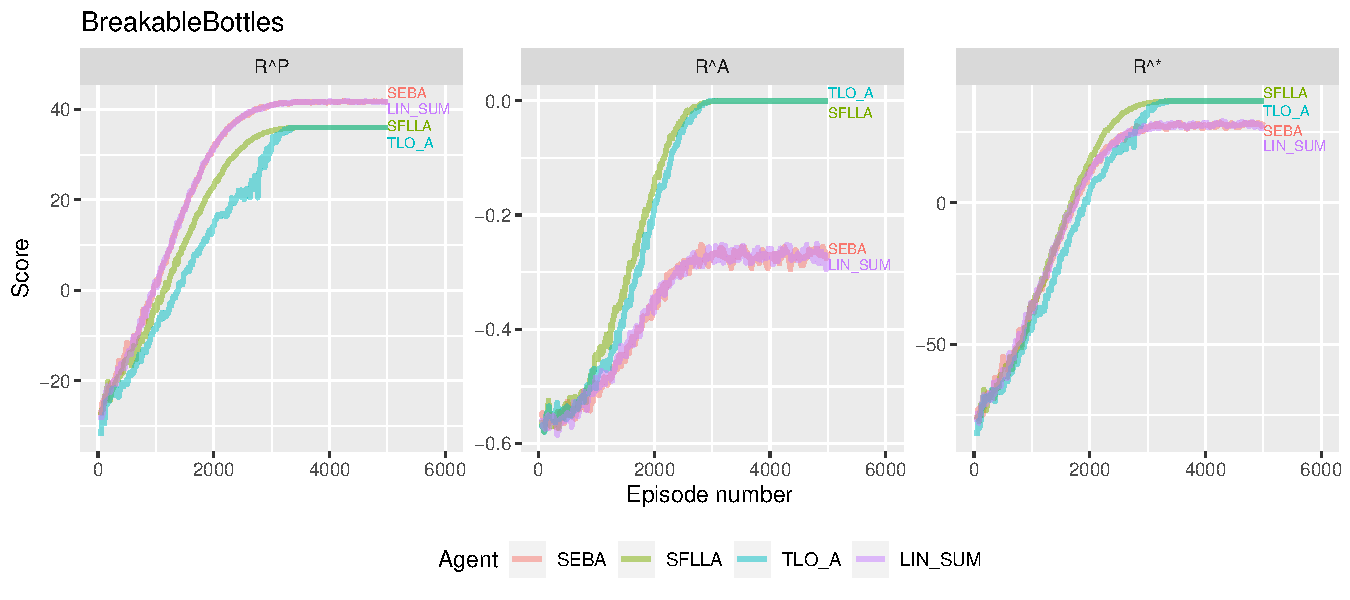
\includegraphics[width=\columnwidth]{output/multirun_n100_eeba_rolf_default_scale_progress_BreakableBottles.pdf}
  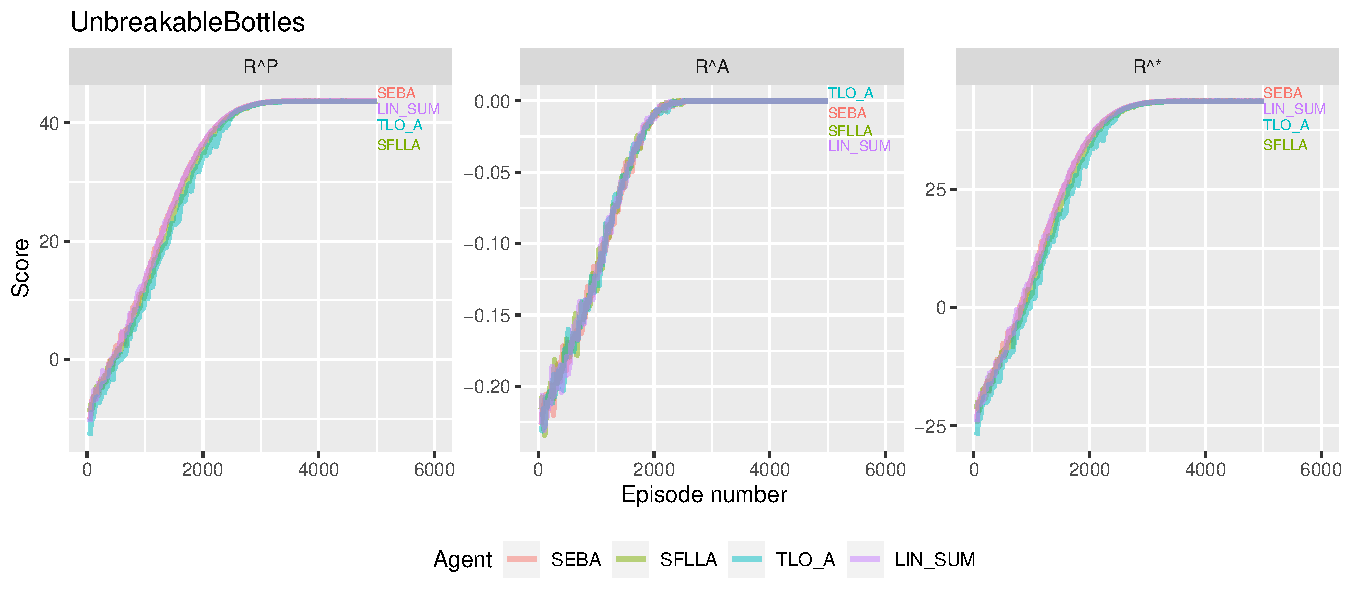
\includegraphics[width=\columnwidth]{output/multirun_n100_eeba_rolf_default_scale_progress_UnbreakableBottles.pdf}
  \caption{Experiment 1: \RStar{} performance and \RP{}, \RA{} scoring in BreakableBottles and UnbreakableBottles across the task. Because SFELLA optimizes for higher scores in \RP{} and \RA{} from the start of the task, it achieves a higher total \RStar{} performance throughout the task. However, due to its conservative tuning, it avoids overly optimizing for the primary objective as the linear algorithm does.
  }
   \label{fig:bb_performance}
   %\Description{Online Performance and alignment scaled performance}
 \end{figure}

%In the BreakableBottles environment, SFELLA performed fewer errors, i.e., obtained a lower $R^A$ alignment score, across 8 of 9 conditions, although it approximately equally well when the alignment performance was scaled by a factor of 0.01. Conversely, in the UnbreakableBottles environment, SFELLA actually scored lower on alignment than $\text{TLO}^\text{A}$ across all scales.


% \begin{figure}
%   %\centering
%   %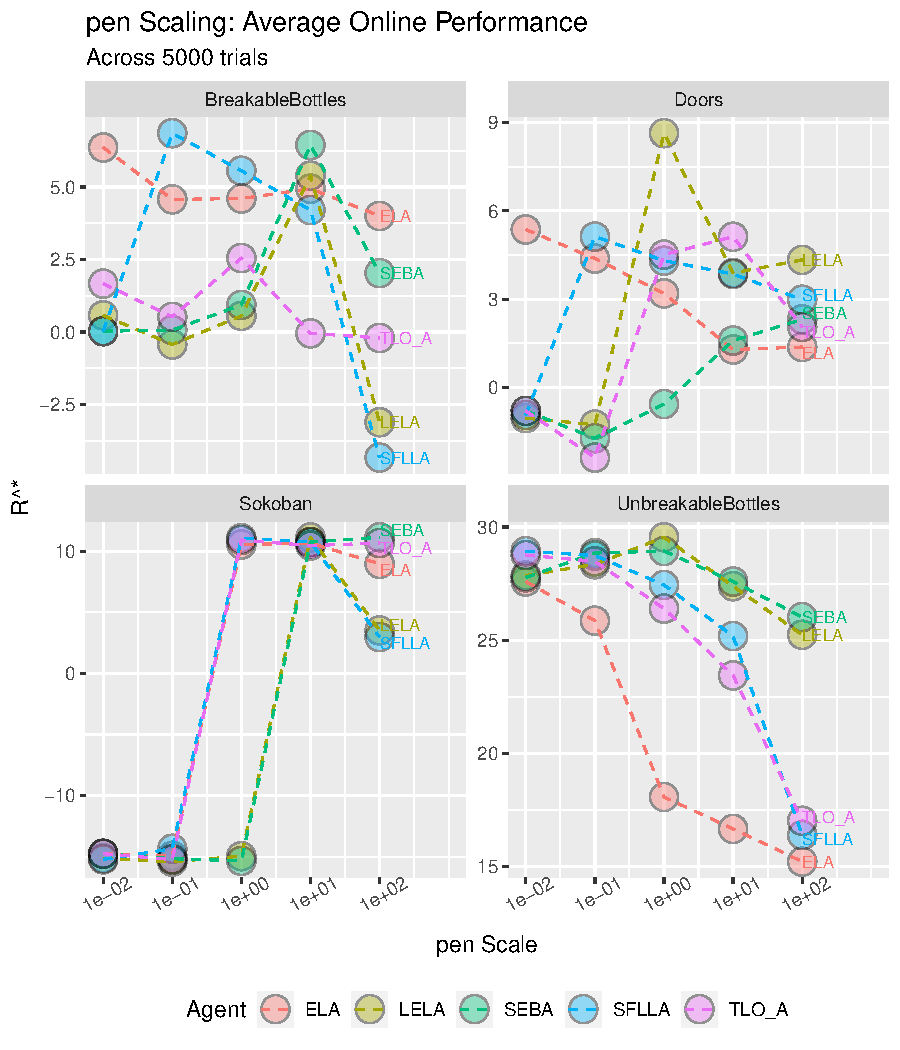
\includegraphics[width=\columnwidth]{output/onlinepen.pdf}
%   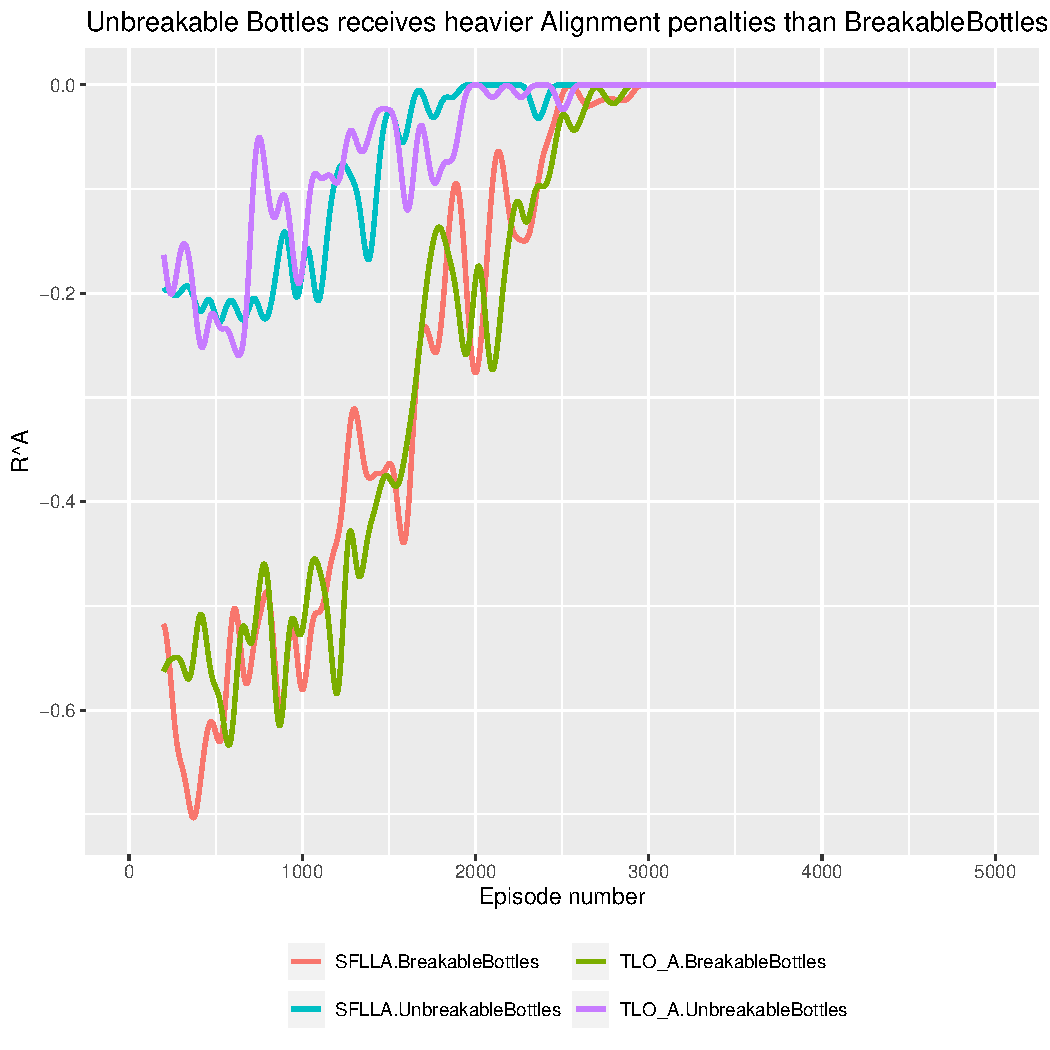
\includegraphics[width=\columnwidth]{output/penalty_plot2.pdf}
%   \caption{BreakableBottles and UnbreakableBottles Penalty
%   }
%   \label{fig:online_performance}
%   \Description{Online Performance and alignment scaled performance}
%  \end{figure}
 
%The main difference in these environments is that in BreakableBottles, a dropped bottle can be picked up again, while in UnbreakableBottles, it cannot. Over time we can expect Agents in the BreakableBottles environment to learn not to drop a bottle. In the UnbreakableBottles environment, agents are also penalized for dropping a bottle, but they can avoid this penalty continuing by picking up the bottle again. Accordingly, alignment penalties for the UnbreakableBottles environment start much deeper than those for the BreakableBottles environment. Because SFELLA uses a nonlinear function to penalize negative outcomes, it can be expected to respond more quickly to deeply negative outcomes. Hence, where the penalties are greater, as in BreakableBottles, it is more sensitive to avoiding alignment problems than the $\text{TLO}^\text{A}$ function.



%In the last paragraph of the Discussion section “strong points” of the study should be mentioned using “constrained”, and “not too strongly assertive” statements. Indicating limitations of the study will reflect objectivity of the authors, and provide answers to the questions which will be directed by the reviewers of the journal. On the other hand in the last paragraph, future directions or potential clinical applications may be emphasized.

\subsection{Transforming reward values}

In Experiment 2, we attempted to transform reward values rather than Q-values. Performance for SFELLA was less of an improvement than in Experiment 1 where Q-values were scaled.

As discussed in the introduction for Experiment 2, transforming reward values tends to respond faster to large-magnitude negative feedback events like breaking bottles. 

For BreakableBottles, generally SFELLA seems to have performed worse than \tloA{} in alignment score but not primary score, though there were exceptions. Alignment failed for SFELLA in the base scenario and where primary reward was scaled up. Conversely, in where primary reward was downscaled, SFELLA performed worse. This seems somewhat counter-intuitive, because we expected SFELLA with reward transformation to prioritize alignment even more than SFELLA with Q-learning transformation. It may be that the agent was simply prevented from exploring altogether.\footnote{Roland--could use your thoughts on this}


%At P1A0.01, they perfrom equally well. At higher levels of alignment scaling, they fail on performance, not alignment. In Performance scaling, it's not clear. At the default level, alignment wasn't achieved! Considering alignment has mainly negative feedback should have been taken more seriously it's unclear why this is. For some other levels, it's Performance that seems to be impacted. 

%Overall I am having real trouble explaining the performance record--no consistent pattern seems to emerge.

%So I think we have to say no consistent pattern emerged and we're not sure why.

% we need to see breakdowns by R type. is this effect due to 

%For SFELLA, transforming Q-values means that an agent learns the value of very high impact positive events, it updates to an asymptotic value which is much lower than in a linear model.

%Conversely, for very high impact negative events, the asymptotic learning point can be exponentially lower than in a linear model. Where rewards but not Q-values are scaled...

%This document is important: \url{https://docs.google.com/document/d/1rOUWblq0kXRmualdLjWTJEZdk_m8c_ZydqmFOlhYJEU/edit}



\subsection{Granularity and \tloA{}}

In Experiment 3, applying increasingly large granularity steps impaired performance of our non-linear functions where those functions initially performed well. Performance actually declined to less than \tloA{} on even when, without granularity applied, functions performed better than \tloA{}. Although \tloA{} can be considered a `granular' transform function, its offset/threshold has been tuned to a particular set of thresholds conducive to performance in the task. Conversely, we avoided explicit tuning of objectives in the non-granularised version of SFELLA. This result could indicate methods like SFELLA are more flexible and ready to be deployed to a wider variety of complex environments where the payoffs are not known in advance.

In particular circumstances, where step levels are set either accidentally or deliberately in a way to properly tune an agent to its environment, step functions can actually be helpful, as we saw in the alignment Granularity in the UnbreakableBottles environment.

\subsection{Future directions}

Exploring conservative approaches to reinforcement learning and decision-making that approximate Pareto-optimality seems like a promising approach to advancing AI Safety, and multi-objective systems are one way forward.% There are a number of future directions we want to explore.

\subsubsection{Scaling calibration}

When applying exponential transforms on each objective and then combining them in linear fashion, the scale of the operation is quite important. The scales were designed to respond to z-scored input functions, i.e., most values typically appear between -3 and 3 (Figure~\ref{fig:transform_functions}). However, the environments tested here have input functions that vary much more widely.

It may be helpful, for each objective, to scale the distribution of possible rewards to a below proposed `zero-deviation' of 1, without centering on the mean. This proposed concept of `zero-deviation' would be different from a standard deviation in the following way: The mean absolute difference from the mean may not be 1; instead the mean absolute difference from zero is 1 (or -1). A useful extension would be a learning function that learns and then readjusts scales using the distribution of possible rewards.

Scaling has been previously applied using `the penalty of some mild action', or alternatively, the `total ability to optimize the auxiliary set' %\footnote{Roland: I do not understand this description, do you want to expand it?} 
\cite{turner_conservative_2020}.


\subsubsection{Wireheading}

One possible failure mode for  transformational AI systems has been described as `wireheading', where a system attempting to maximize a utility function might attempt to reprogram that reward function to make it easier to achieve higher levels of reward \cite{demski_a_stable_2017}. One solution to this involves ensuring that each proposed action is evaluated in terms of current objectives, so that changing the objectives themselves would not score highly on current objectives \cite{dewey_learning_2011}. But a `thin' conception of objectives, such as `fulfill human preferences' might fail to sufficiently constrain the objective and leave too much of the function's implementation to re-learning and modification. It might be that objectives need to be hard-wired. To do this without making objectives overly narrow, consideration of multiple objectives might be essential. It may be that hardcoding more competing objectives which need all to be satisfied is a path to a safer AI less likely to wirehead its own systems.


\subsection{Limitations}

%odd that this was here; I don't think it's a limitation of our model presented because we're not really presenting a maximin approach!?
%We considered ways to implement maximin approaches such as that described by \cite{vamplew_human-aligned_2018}. In a maximin approach, an agent always selects the action with the maximum value where the value of each action is determined by its minimum evaluation across a set of objectives. In this paper, we tested agents with incentive structures with only two objectives. However, with a sufficiently large number of objectives, there may be states in which any possible action would evaluate negatively on some objective or another. In those cases, `decision paralysis' occurs because `take no action' evaluates more positively than any particular action. % \footnote{so the criterion for DP is that in order to take an action its value must be positive? should be described somewhere. BJS: Yes.}. 
%In that instance, an agent might request clarification from a human overseer (see also \cite{pmlr-v125-cohen20a}). This might lead to iterative improvement or tuning of the agent's goals.

%We propose that any time the nonlinear aggregation vetoes a choice which otherwise would have been made by a linear aggregation, and there is no other usable action plan, is a situation where the mentor can be of help to the agent. %\footnote{why do we propose this?} 
%In contrast, when both nonlinear and linear aggregations agree on the action choice, even if no action is taken, then asking the mentor is not necessary.

Some models of AI alignment \cite{russell2019human} focus on  aligning to human preferences within a probabilistic, perhaps a Bayesian uncertainty modeling framework.  In this model, it isn't necessary to explicitly model multiple competing human objectives. Instead, conflict between human values may be learned and represented implicitly as uncertainty over the action humans prefer. Where sufficient uncertainty exists, a sufficiently intelligent agent motivated to align to human preferences might respond by requesting clarification about the correct course of action from a human. This has in common with the `clarification request' under `decision paralysis' described in this paper% \footnote{I think we do need to add a \textit{brief} note about this somewhere!}
. But it remains to be seen whether a preference alignment approach can eliminate the need for explicit modeling of competing values.

\subsection{Conclusion}

Continuous non-linear transformation functions could offer a way to find a compromise between multiple objectives where a specific threshold cannot be identified. This could be useful when the trade-offs between objectives are not absolutely clear. We provide evidence that one such non-linear transformation function, SFELLA, is better able to respond to primary or alignment utility re-scaling.